%% ****** Start of file template.aps ****** %
%%
%%
%%   This file is part of the APS files in the REVTeX 4 distribution.
%%   Version 4.0 of REVTeX, August 2001
%%
%%
%%   Copyright (c) 2001 The American Physical Society.
%%
%%   See the REVTeX 4 README file for restrictions and more information.
%%
%
% This is a template for producing manuscripts for use with REVTEX 4.0
% Copy this file to another name and then work on that file.
% That way, you always have this original template file to use.
%
% Group addresses by affiliation; use superscriptaddress for long
% author lists, or if there are many overlapping affiliations.
% For Phys. Rev. appearance, change preprint to twocolumn.
% Choose pra, prb, prc, prd, pre, prl, prstab, or rmp for journal
%  Add 'draft' option to mark overfull boxes with black boxes
%  Add 'showpacs' option to make PACS codes appear
%  Add 'showkeys' option to make keywords appear
\documentclass[aps,prl,preprint,groupedaddress]{revtex4}
%\documentclass[aps,prl,preprint,superscriptaddress]{revtex4}
%\documentclass[aps,prl,twocolumn,groupedaddress]{revtex4}
\usepackage{graphicx}
\usepackage{mathtools}
\usepackage{fancyref}
\usepackage{float}
\usepackage[utf8]{inputenc}

% You should use BibTeX and apsrev.bst for references
% Choosing a journal automatically selects the correct APS
% BibTeX style file (bst file), so only uncomment the line
% below if necessary.
%\bibliographystyle{apsrev}

\begin{document}

% Use the \preprint command to place your local institutional report
% number in the upper righthand corner of the title page in preprint mode.
% Multiple \preprint commands are allowed.
% Use the 'preprintnumbers' class option to override journal defaults
% to display numbers if necessary
%\preprint{}

%Title of paper
\title{Towards Entropic Trapping of DNA in Solid-State Nanopores}

% repeat the \author .. \affiliation  etc. as needed
% \email, \thanks, \homepage, \altaffiliation all apply to the current
% author. Explanatory text should go in the []'s, actual e-mail
% address or url should go in the {}'s for \email and \homepage.
% Please use the appropriate macro foreach each type of information

% \affiliation command applies to all authors since the last
% \affiliation command. The \affiliation command should follow the
% other information
% \affiliation can be followed by \email, \homepage, \thanks as well.
\author{Lucas Eggers}
%\email[]{Your e-mail address}
%\homepage[]{Your web page}
%\thanks{}
%\altaffiliation{}
\affiliation{Brown University}

%Collaboration name if desired (requires use of superscriptaddress
%option in \documentclass). \noaffiliation is required (may also be
%used with the \author command).
%\collaboration can be followed by \email, \homepage, \thanks as well.
%\collaboration{}
%\noaffiliation

\date{\today}

\begin{abstract}
% insert abstract here
\end{abstract}

% insert suggested PACS numbers in braces on next line
\pacs{}
% insert suggested keywords - APS authors don't need to do this
%\keywords{}

%\maketitle must follow title, authors, abstract, \pacs, and \keywords
\maketitle

% body of paper here - Use proper section commands
% References should be done using the \cite, \ref, and \label commands
\section{Introduction}

Better nanofluidic control over DNA will yield exciting leaps in technology, such as biochemical labs-on-a-chip and so-called DNA hard drives.
We intend to get a few steps closer by making an isolation chamber to hold single DNA molecules in place.
Such an isolation chamber would allow for the outcome of biochemical experiments to be observed on a per-molecule basis.
It could also act as a storage medium for data encoded in DNA which can hold the equivalent of one million CDs in a single gram for 10,000 years\cite{dna-hard-drive}.
We believe we can create such an isolation chamber based on entropic trapping, and combine it with a molecular detector called a nanopore.

In order to isolate a single DNA molecule in the chamber, we need a way to deliver it and to know when it enters.
Nanopores are the ideal device for such purposes.
A nanopore is a small hole in a membrane, be it biological or synthetic.
Solid-state nanopores consist of a hole approximately 10 nanometers across in some larger solid-state membrane.
For contrast, double-helical DNA is approximately 2.5 nanometers across.
When placed between two reservoirs of ionic solution, solid-state nanopores can detect the passage of a single DNA molecule.
This passage event is also known as a translocation.
When a voltage bias is placed across the two reservoirs, current forms from ions flowing through the pore.
DNA, driven by electrophoretic forces on its slight negative charge, travels toward the pore, eventually getting sucked through.
Its passage displaces some flowing ions, causing an observable drop in the ionic current through the pore.

In order to trap DNA in its isolation chamber, we intend to take advantage of the DNA’s configurational entropy.
At equilibrium, DNA forms a random coil whose spherical shape has a size characterized by the radius of gyration (Rg).
If we could get DNA in a cavity that is roughly the size of the radius of gyration and that has holes smaller than the radius of gyration on either side, we predict that the molecule will have a near-zero probability of diffusing out; it would have to squeeze too far out of equilibrium to exit this entropic trap.\cite{trapping}

\begin{figure}
\centering
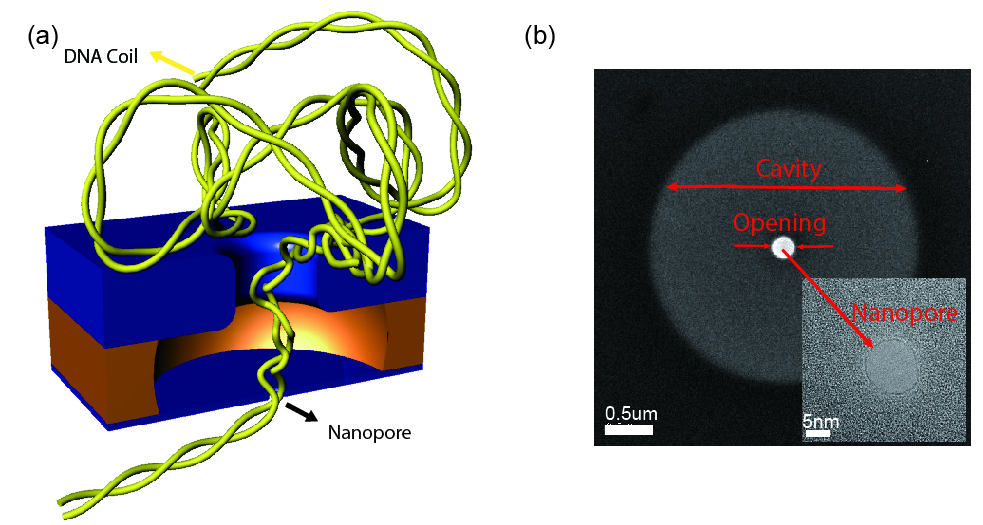
\includegraphics[width=.4\textwidth]{figures/nanopore-schematic}
\caption{A schematic of a silicon structure containing a nanopore and adjacent chamber during a DNA translocation event.
The structure has 3 main layers.
From bottom to top they are the nanopore, the cavity, and a large hole with diameter 500nm on average.}
\label{fig:nanopore-schematic}
\end{figure}

The device we envisioned to trap individual DNA molecules is shown in Fig.~\ref{fig:nanopore-schematic}.
(Note that the molecule pictured is not trapped.) Capturing a DNA molecule in the cavity can be thought of as a competition between two timescales: the time required to push the center of mass of the DNA through the structure and the time it takes the DNA molecule to equilibrate in the cavity so it cannot traverse the large hole.
A translocation starts when the leading tip of DNA  - or someplace nearby on the polymer - enters the nanopore.
A drop in current is observed.
The molecule is driven through the cavity by local electric fields.
As it is driven, Brownian motion causes the molecule to start to equilibrate and expand to fill the chamber.
However, translocation happens much faster than equilibration, so the molecule remains ``skinny'' when compared to the large hole; continuing to push it will cause it to exit the structure.
Thus, the probability of exit is dependent on the cavity length and hole diameter.
When the molecule finishes translocating the current will return to its original baseline value.
Turning off the driving voltage at the right moment will allow the molecule to equilibrate inside the cavity, trapping it.

Placing such a structure between two reservoirs of ionic solution yields the translocation dynamics described above with a twist: the structure’s asymmetry means translocations from either side of the pore are not equivalent.
Although the effects of the asymmetric structure on translocation dynamics will be touched on, Karri DiPetrillo's thesis takes a deeper look at those phenomena.
The focus of this thesis will be trapping DNA molecules approaching the exposed nanopore (the bottom layer in Fig.~\ref{fig:nanopore-schematic}).
Our objectives are thus twofold: to develop the hardware (pores-plus-chambers) and the software (control electronics and data analysis) to make our vision a reality.
My contributions were software for analysis and recommendations for programming control electronics informed by my preliminary experiments and theoretical calculations.
In addition to creating more intricate labs-on-a-chip as in \ref{fig:trapped-and-snipped} and possibly storing DNA hard drives, creating such entropic traps would yield deeper understanding of DNA as a polymer more generally.

\begin{figure}
\centering
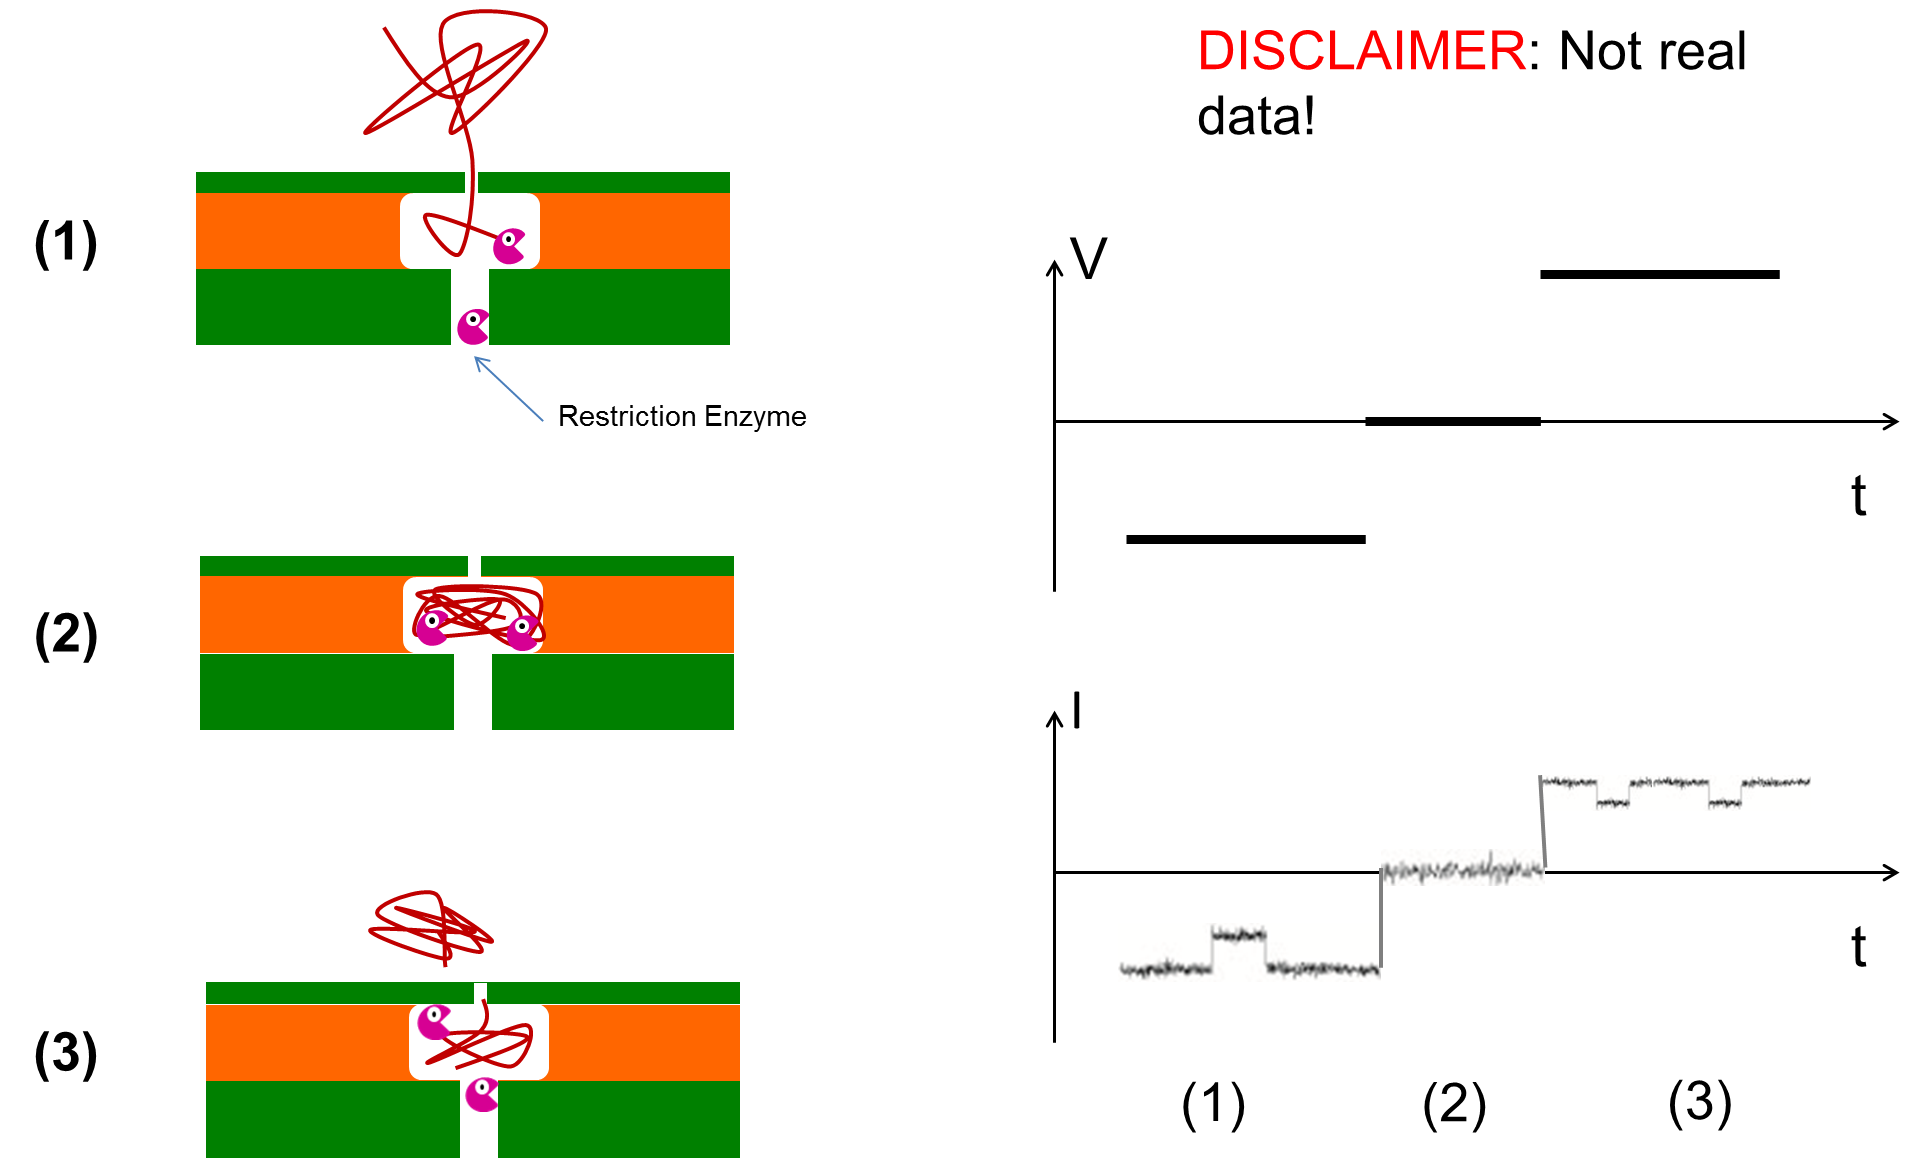
\includegraphics[width=1\textwidth]{figures/idealized-trapping}
\caption{An idealized lab-on-a-chip in which an entropic trap would effectively be a nanoscale test tube. We should be able to trap a DNA molecule by turning off voltage at the proper time (1), perform some biochemistry on it (such as segmenting it using a restriction enzyme) (2), and test whether our chemistry proceeded as planned by using the detection properties of the nanopore (3).}
\label{fig:trapped-and-snipped}
\end{figure}
% Put \label in argument of \section for cross-referencing
%\section{\label{}}
\section{Theory}

\subsection{Quantifying DNA as a Polymer}

We know the molecule can be entropically trapped when \(R_g\) is greater than the constraining length, in our case the large hole opposite the nanopore.
The expanded, randomly (coiled, configured?) molecule at equilibrium would have to squeeze itself in an energetically unfavorable way to fit through the large hole.\cite{trapping}
The molecule equilibrates to \(R_g\) in a characteristic time we also need to know to asses the feasibility of trapping;
\(R_g\) does not matter if the molecule has already passed the constraining feature of the structure before it equilibrates.
We used linearized \(\lambda\)-DNA in our experiments so I will use its properties to get values in units like meters and seconds from equations.

In the simplest models of polymer statistics at equilibrium we consider only two properties of the molecule: its total length \(L\) and persistence length \(l_p \ll L\).
\(l_p\) can be thought of as a measure of the stiffness of the molecule.
These two numbers describe a freely-jointed chain of length \(L\) in which rigid lengths of polymer of size \(p\) are connected by joints that can take any bond angle.
The resulting shape of such an object is a sphere.
Mathematically the chain can be described by a three-dimensional random walk.
As such, one would expect the radius of the sphere, also known as the radius of gyration, to scale with the square root of the length of the chain: \(R_g \propto L^{1/2}\).
The flaw in such reasoning is that real polymers are self-avoiding, meaning that links in the chain cannot occupy the same space.
The Flory model modifies the random walk by using a mean field approach (where segments encounter one another with equal probability) to define a new parameter, the Flory exponent \(\nu_F\), where \(R_g \propto L^{\nu_F}\).
The Flory model predicts that, for DNA, \(\nu_F = \frac{3}{5}\).
Simulations and experiments yield an exponent of approximately .588.\cite{exponent}
For \(\lambda\)-DNA \(R_g\) is \(0.73\mu\)m.
To make the Flory model even more realistic, we must take into account Brownian motion.
The Rouse model describes a polymer as a collection of beads connected by springs in which beads feel the effects of thermal forces and drags.
It does not, however, take into account self-avoidance and as such is more useless than the Flory model. 

Timescales are provided by the Zimm model.
Zimm combined the Flory and Rouse models by including the hydrodynamic interactions between different parts of the chain as mediated by the solvent.
The Zimm model's predictions most exactly agree with experiment. The Zimm model predicts that a polymer enters its equilibrium state from any other state within a characteristic relaxation time \(\tau_z\).
That is, if one stretched a DNA molecule to be completely straight, it would reach a spherical conformation in \(\tau_z\) seconds, maximum.
The process of reaching such a sphere is known as relaxation.
For \(\lambda\)-DNA \(\tau_z \approx 100\)ms.
Our translocations last \(\approx 2\)ms, so molecules do not have time to equilibrate until long after they translate.
Thus our translocations are called ``fast translocations.'' To paint a physical picture of what that means, we imagine a randomly coiled rope being pulled off a table.
As it is pulled, individual folds are sequentially straightened and pulled off the table.
Only a small length of rope (the most recently straightened fold) is involved in the motion.
The rest of the rope is stationary.
The same things happens with DNA, but at approximately $10^{-7}$ of the rope's length scale.
Folds of the molecule are sequentially straightened as they are sucked through the pore while the rest of the molecule is effectively frozen.

\subsection{Trapping in More Detail}

Trapping can be thought of as a competition between the movement of DNA through the pore-plus-cavity structure and the equilibration of the molecule in the cavity.
The major force pushing the DNA molecule though the structure is electrophoretic.
From charge conservation we know that, to a good approximation, the current traveling through the pore (our measured quantity) is equal to the current passing through the area of hemisphere enclosing the pore: 
\begin{equation} I = 2 \pi R^2 J(R) \label{eq:constant-current}\end{equation} 
where \(I\) is current, \(R\) is distance from pore, and \(J(R)\) is the current density.
Solving Eq.~\ref{eq:constant-current} for \(J(R)\) we see 
\[J(R) = \frac{I}{2 \pi R^2}.\] 
By Ohm's Law we know 
\[\overrightarrow{J}(R) \equiv \sigma \overrightarrow{E}(R),\]
where \(\sigma\) is two-dimensional charge density.
Combining these equations and solving for E yields:
\begin{equation} E(R) = \frac{I}{\sigma 2 \pi R^2} \label{eq:electric-field} \end{equation} 
We know the velocity of the DNA molecule a distance \(R\) from the pore: 
\begin{equation} v_{\mathrm{DNA}} = \mu_{\mathrm{DNA}} E(R) \label{eq:velocity} .\end{equation} 
Plugging in Eq.~\ref{eq:electric-field} we see that
\[v_{\mathrm{DNA}} = \frac{\mathrm{d}R}{\mathrm{d}t} = \mu_{\mathrm{DNA}} \frac{I}{\sigma 2 \pi R^2},\]
where \(\mu_{DNA}\) is the electrophoretic mobility of DNA.
Integrating yields the tip's distance from the pore and the elapsed time:
\[\int_{R=0}^{R(\Delta t)} \frac{\sigma 2 \pi R^2}{\mu_{\mathrm{DNA}} I} \mathrm{d}R = \int_{t=0}^{\Delta t} \mathrm{d}t \]
yields an equation
\[\frac{1}{3} \frac{\sigma 2 \pi R^3}{\mu_{DNA} I} = \Delta t,\]
which can be solved for \(R(\Delta t)\):
\begin{equation} R(\Delta t) = \sqrt[3]{\frac{3 \mu_{DNA} I}{\sigma 2 \pi}\Delta t} .\label{eq:competition}\end{equation}
Eq.~\ref{eq:competition} quantifies the location of the tip as a function of time.
If \(R(\Delta t)\) is less than the height of the cavity, the molecule should be trapped.
Even if the tip could travel outside of the chamber (that is, \(R(\Delta t)\) greater than cavity height), we believe the molecule will still be trapped with high probability if the center of mass is within the cavity.
The center of mass, the point from which \(R_g\) is measured, should be at approximately \(R(\Delta t)/2\).
The major assumption in this calculation is that current is conserved across a hemispherical geometry within the cavity.
That may be true to a first approximation, but in reality all current must flow through the hole at the other end of the structure and thus the fields are ``squeezed'' into that hole; the molecule will travel slightly farther than expected as it reaches the far side.

Now we will find an actual value for cavity size.
Plugging in numbers from our experiments, \(\mu_{DNA} = 3.75 \times 10^{-3}\)cm$^2$/V$\cdot$s, \( = 3.75 \times 10^{-7}\)m$^2$/V$\cdot$s \cite{mobility} \(I = 20 \mathrm{nA} = 2\times 10^{-8}\mathrm{A}, \Delta t = 2\mathrm{ms} = \mathrm{ms} = 2 \times 10^{-3}\)s and \(\sigma = 100\)mS/m = 10 S/m\cite{CRC}, we see that the molecule travels \[R(\Delta t) = \sqrt[3]{\frac{3 \mu_{DNA} I}{\sigma 2 \pi}\Delta t} = \sqrt[3]{\frac{3\cdot 3.75\times 10^{-7}\cdot 2\times10^{-8}}{10\cdot 2\cdot \pi} 2\times10^{-3}}\] \[\approx 8.95 \times 10^{-7}\mathrm{m} = 895 \mathrm{nm} \] in the time it takes to translocate.
Half of this (that is, 450nm) gives us a lower bound for cavity length.
Because our cavities were roughly \(400\)nm long and we did not kill the voltage immediately after translocation, we captured no DNA molecules in our preliminary trials.
We now understand why and are seeking to fabricate devices with longer chambers and build and program better control electronics to improve responsiveness.


\section{Experiment}

\subsection{Synthesis of Nanopores}

[where do i put the fact that i worked with karri? in attributions at the end or what?]
We fabricated our nanopore-plus-cavity structures to entropically trap DNA molecules using methods similar to Zandbergen et al.\cite{nanopore-fabrication}
We start with large wafers with the layers seen in Fig.~\ref{fig:structure-schematic} manufactured by the Cornell Nanofabrication Facility.
We first use two types of etching to burn through the top two layers of the wafer to gain access to layers in which we make more interesting structures.
The top layers are present due to constraints of the manufacturing process.
We first use thermal plasma etching to remove the top silicon nitride layer followed by potassium hydroxide base to remove the pure silicon.
We then use a Focused Ion Beam (FIB) to create holes in the middle layer of SiN with diameters ranging from 150 to 900 nanometers and height 400nm.
This diameter is the constraining feature of the setup that entropically traps DNA.
The FIB hole allows access to the silicon oxide layer which is etched using hydrofluoric acid, creating a chamber 1-2\(\mu\)m in diameter and 400nm tall in the our experiments.
Recent wafer orders have a taller layer of silicon oxide, enabling us to make taller chambers.
Last, but not least, we create the nanopore in the final layer of silicon nitride roughly 10nm in diameter and 20nm tall using a Transition Electron Microscope.
This novel structure is ideal for entropic trapping because it places the cavity that will trap the molecule directly adjacent to the molecular detector.
Thus we can necessarily know when a candidate for trapping enters the chamber.

\begin{figure}
\centering
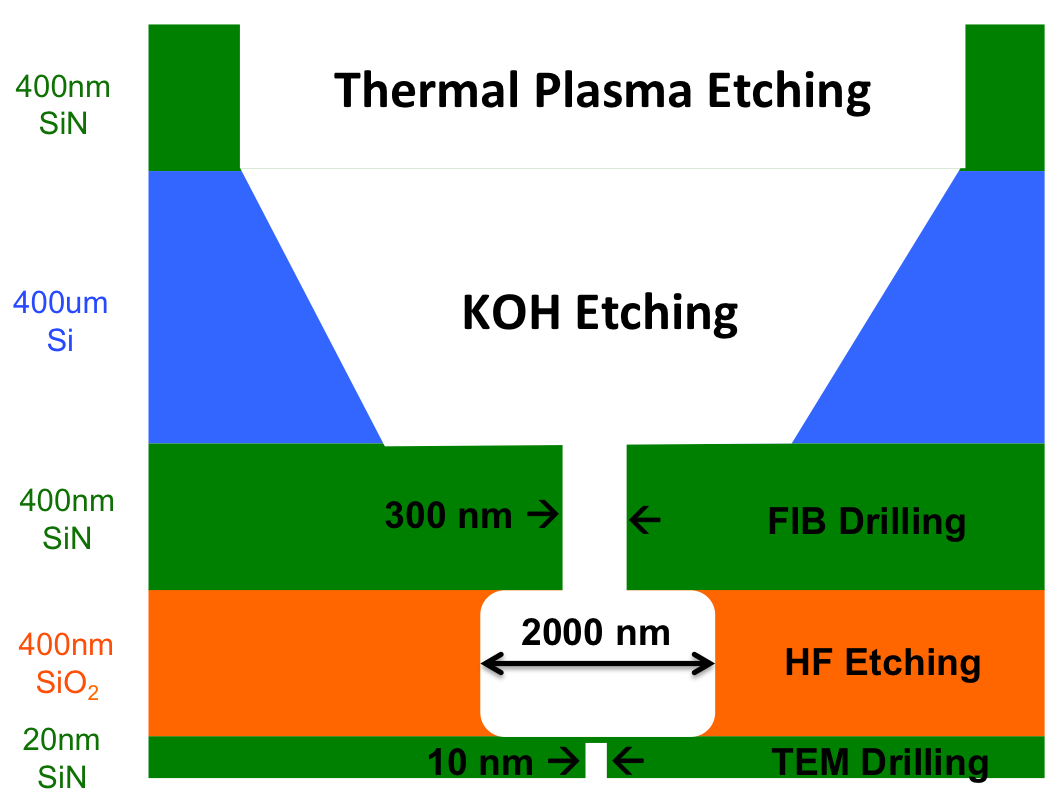
\includegraphics[width=.45\textwidth]{figures/structure-schematic}
\caption{A more specific schematic of our structure including methods of feature creation. Note: Not to scale.}
\label{fig:structure-schematic}
\end{figure}

\subsection{Apparatus and Setup}

Nanopores are excellent single-biomolecule detectors.
As such, we needed to take steps to ensure that the only biomolecules present in our experiments were DNA.
To remove all foreign contaminants (things like skin cells, dust, possibly hair) we cleaned our nanopores in Nano-Strip (Cyantek  Corporation, 90\% sulfuric acid, 5\% peroxymonosulfuric acid, 5\% water) at 75$^\circ$C for 2.5 hours.
Nano-Strip also made our pores hydrophilic which helped reduce noise in our data.
Pores were then rinsed with deionized water and placed in a custom-made PVC chuck pictured in Fig.~\ref{fig:chuck}.
We rinsed the setup by pushing degassed, deionized water and isopropyl alcohol through the fluid inlets.
We then prepared to add DNA to the setup by filling reservoirs with a millipore-filtered, degassed buffer solution of 1M KCl, 10mM Tris-HCl and 1mM EDTA buffer with pH 8.0.
We placed the chucks in Faraday cages, plugged in the electrodes, and turned on our data collection equipment.
To establish a control baseline - typically around 15nA - we applied a 100mV voltage bias across the pore and began recording.

To record data we used an Axon Axopatch 200B high-speed electrometer which converts the analog signals received from the elctrodes into digital, numerical values.
We sampled the analog signal at a rate of 250kHz.
To control voltages we used a National Instruments SCB-68 field-programmable gate array (FPGA) card.
FPGAs are designed to be customized with machine description code after purchase to implement complex computations on-the-fly.
They feature plentiful computation and fast-access memory resources to ensure computations and their requisite reactions are executed as quickly as possible.

\begin{figure}
\centering
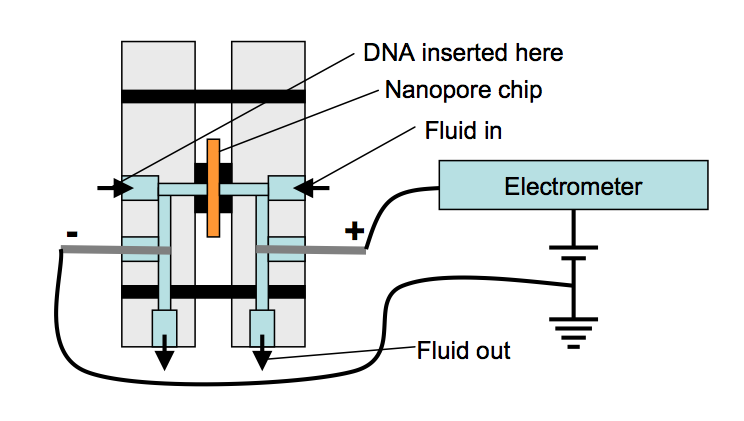
\includegraphics[width=.6\textwidth]{figures/chuck}
\caption{A schematic of translocation experiment setup. (Taken from Nick Hagerty's thesis.)}
\label{fig:chuck}
\end{figure}

\subsection{Procedures}

We added DNA to our setup by filling the reservoirs with the same buffered solution as above with the addition of linearlized $\lambda$-DNA (48.5kbp, New England Biolabs) diluted to a concentration of 500ng/ml.
This setup generalizes well to multiple types of nanopore experiment; changing experiments requires only changing the code of the FPGA.

\subsubsection{Monodirectional Translocations}

A typical monodirectional translocation experiment involves the application of a constant driving voltage for a predetermined experimental duration.
We applied voltages ranging from 140mV to 60mV in 20mV steps biased in both directions for 10 minutes each.
In these experiments the FPGA card did nothing; all voltages were set by hand.
The exact order of tested voltages varied per-experiment but both polarities were run before moving to the next voltage.
A typical minute of collected data is shown in Fig.~\ref{fig:trans-data}.
\begin{figure}[h]
\centering
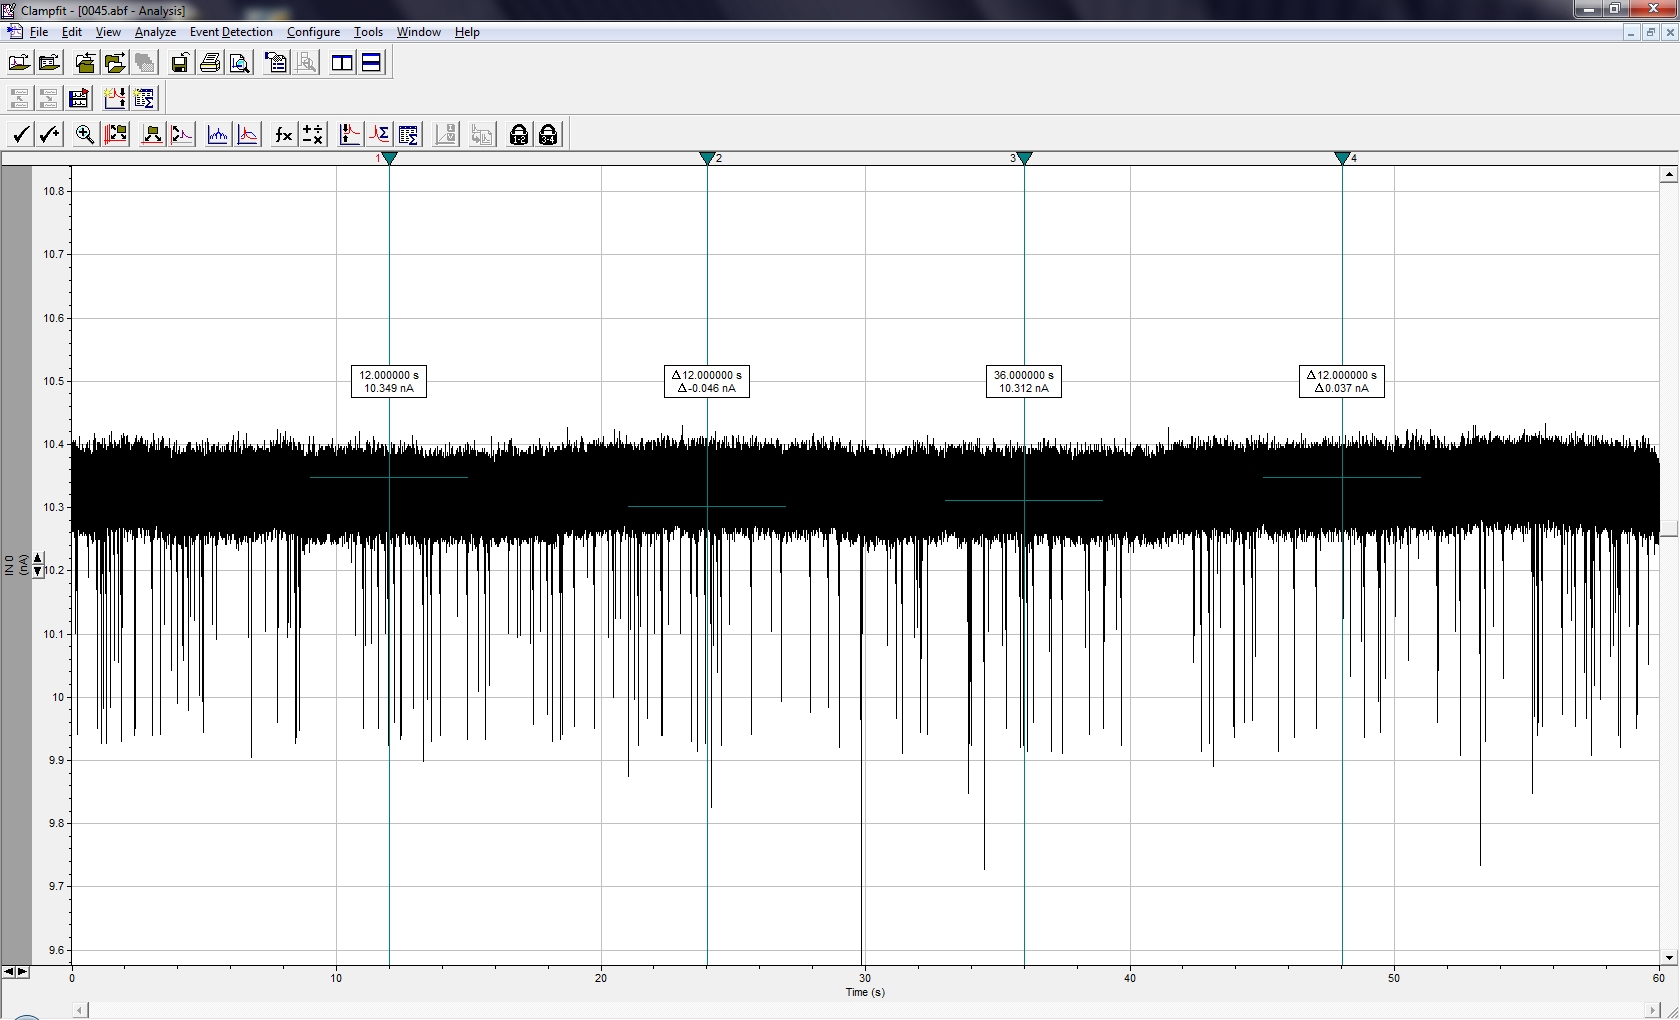
\includegraphics[width=1\textwidth]{figures/monodirectional-minute}
\caption{A typical minute of monodirectional translocation data.
Notice the current scale, noise, slightly unstable baseline and brevity of translocation events.}
\label{fig:trans-data}
\end{figure}

\begin{figure}
\centering
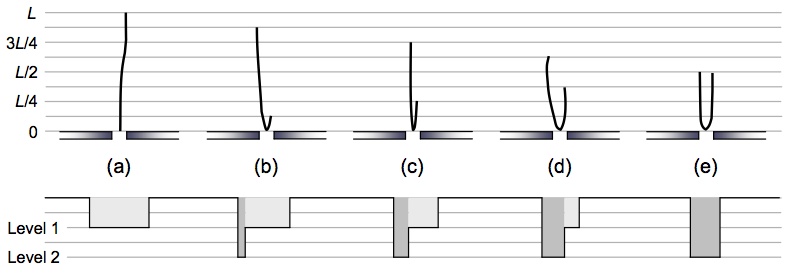
\includegraphics[width=1\textwidth]{figures/dna-approach}
\caption{A schematic of how the stacked-top-hat shape of current vs time data depends on how DNA enters the nanopore. Missing are schematics of multiply-folded molecules but the linear relationship between current blockage and strands in the pore is made clear. Almost every thin spike in \ref{fig:trans-data} is of one of these forms. (Taken from Nick Hagerty's thesis.)}
\label{fig:dna-approach}
\end{figure}

Translocation events look like stacked-top-hat-shaped deviations from the baseline as seen in Fig.~\ref{fig:dna-approach}, indicating a DNA molecule is in the pore displacing ionic current.
Current traces of translocations often feature multiple levels of displacement, indicating the presence of multiple strands of DNA.
Typically multiple strands enter the pore because the DNA molecule is folded; rarely we see fluke events in which multiple DNA molecules translocate together.
Rarer still are knots of DNA molecules that nearly completely block any current from flowing through the pore.
Current can also be blocked by bubbles in solution lodging themselves in the nanopore.
These two types of blockage create drastically different current signatures: bubbles yield a smooth, uninteresting baseline that is much smaller than expected whereas bundled DNA yields an incredibly noisey baseline also much smaller than a clog-free pore.
To dislodge blockages we ``zap'' the system with large voltage spikes and flip the polarity several times in rapid succession.

\subsubsection{Trapping}

Our preliminary endeavors to trap DNA molecules were met with either failure or inconclusiveness.
The procedure followed that of monodirectional translocation experiments except that DNA was placed only on one side of the nanopore.
A voltage (of varying value per experiment) was applied to push DNA across the pore for approximately 30 seconds.
If the pore did not irrevocably clog during the previous step, the polarity of the voltage was then flipped.
We then observed molecules translocating back across the pore!
However, those translocations proved nothing except that it is possible for molecules to stay close enough to the pore to reenter after they have translocated; we had no way of knowing whether or not the molecules were actually trapped.
In fact, given that the molecules were not all recaptured simultaneously we can argue that they were not trapped.
Every time trapping was attempted by manually killing the driving voltage immediately after a translocation the pore was irrevocably clogged.

\subsubsection{``Ping-pong'' Translocations}

The FPGA card played a much larger role in ping-pong experiments.
The experiments began in the same way as monodirectional translocations but diverged as soon as a translocation was observed.
In molecular ping pong, the FPGA measures deviations from the baseline current.
When a molecule is seen translocating, a timer, call it the flip timer, begins counting down from a predefined value between two and ten milliseconds.
When the timer hits zero, the FPGA card flips the polarity of the voltage, hoping to ``recapture'' the most recently translocated molecule.
Recapture here takes a drastically different meaning than one may expect: instead of having anything to do with trapping, recapture refers to the return of a molecule that has recently completed a translocation through the pore.
Ping-pong experiments at present do not use pores with any cavity structure affixed; pores are stripped down to only one nanoscale hole in one layer of silicon.
Upon recapture, another timer, call it the recapture timer, set to a different starting value, begins counting down.
If the molecule is observed translocating again before the recapture timer hits zero, the flip timer begins again and voltage flips again.
This process repeats itself until the recapture timer hits zero, meaning that molecule has finally escaped.
A typical minute of collected data is shown in Fig.~\ref{fig:ping-pong-data} [get a minute of data here]

\subsection{Data Analysis with MatLab}

After collecting current vs. time data at a rate of 250kHz we ran it through our MatLab data analysis pipeline.
Each data file contains one minute of data.
Current, measured in nanoamps, can be positive or negative (depending on driving voltage) but only its absolute value is used in computations to simplify algorithms.
All analysis pipelines start by importing data files (either in pure binary or axon binary file formats) to MatLab-manipulable tables.

\subsubsection{Monodirectional Translocations}

Angus McMullen created the following procedure for analyzing monodirectional translocations during his extensive work with DNA and FD virus.
Xu Liu and I built upon his work to improve our data analysis.
The data analysis for monodirectional translocations starts with data sanitation.
We run once through a given file recording where events start and end.
Our heuristic for detecting translocations in monodirectional experiments is deviation from a baseline value \(\beta\) defined by the moving average of the previous 1ms of data (250 data points).
We average the next 7 points, called the ``lookahead'' or ``EventTest'' \(\Lambda\) and see if it exceeds our threshold for an event.
The last piece of data used to find event boundaries is the root mean square of the baseline \(\Omega = \beta_{RMS}\).
The RMS provides a good measure of the amount of variability, also known as noise, in the baseline.
Each of these values is calculated tens of thousands of times per file as it is traversed from start to end with a step size of \(1/50^{th}\) of a millisecond (5 data points). (dereK: should i break beta and lambda and omega into separated equations and define them that way?)

\begin{figure}
\centering
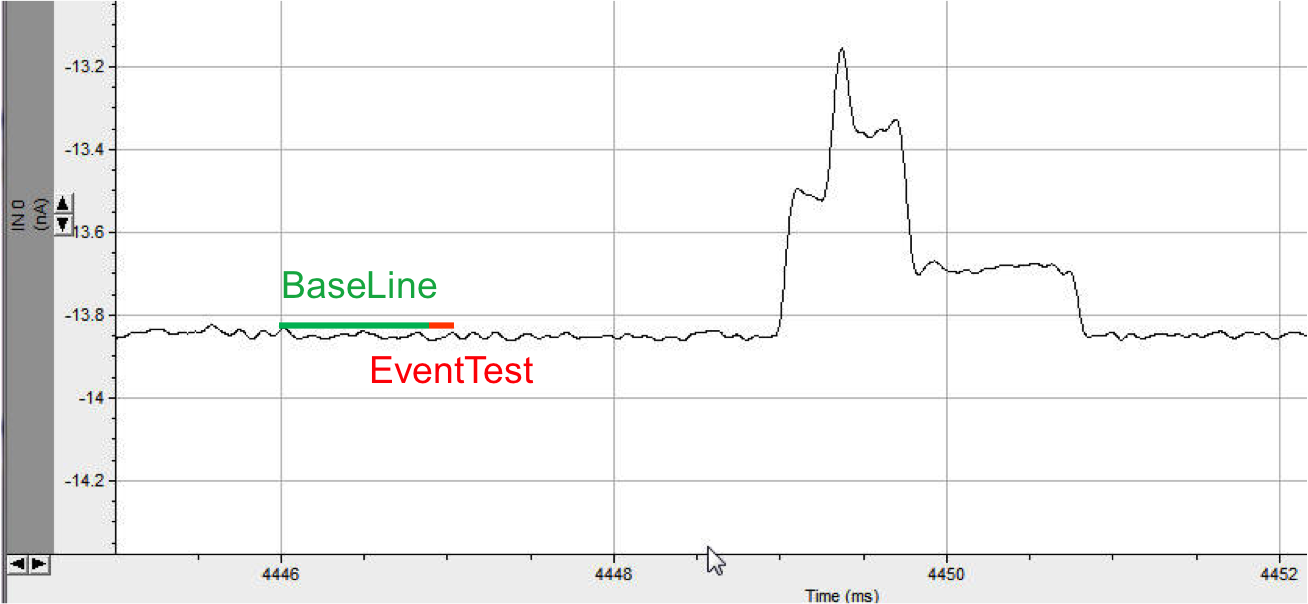
\includegraphics[width=1\textwidth]{figures/find-events}
\caption{A representation of how our MatLab script finds events in monodirectional data. Important features of the data are its relatively static baseline and event structure. The data pictured has been run through a 50kHz software filter for legibility; typical data is much noisier.}
\label{fig:find-events}
\end{figure}

If the lookahead is far enough away from the baseline (``far enough'' \(\Delta\) being dependent on driving voltage and specified by the user, typically a quarter of a nanoamp at 100mV), we know we may have found an event \(\xi\):
\begin{equation} |\beta_{start}| - |\Lambda| \geq \Delta \Rightarrow \xi = \top \label{eq:event-start}\end{equation}
where \(\beta\) is baseline value, \(\Lambda\) is lookahead value, \(\Delta\) is the cutoff value, and \(\xi\) is a boolean value specifying whether we believe we are in an event.
We save \(\beta_{start}\) to use when detecting the end of the event and continue taking the averages \(\beta, \Lambda\) and RMS measurements \(\Omega\) as stated above.
Instead of using a specified threshold as we did when detecting the start of an event, we determine the end of event by checking if the lookahead is greater than the saved baseline minus one tenth of the RMS (remember, all values are positive):
\begin{equation}|\Lambda| \geq |\beta_{start}| - \frac{|\Omega|}{10}. \label{eq:event-end}\end{equation}
The other way an event can ``end'' is by being longer than 20 milliseconds at which point we know that the event flag fired erroneously, likely due to noise or a shifted baseline.
There are two possible extremes for an RMS value to take: the smallest is the noise during an event (which is identical to the noise on the baseline); the largest is if the baseline spans multiple current blockage levels.
We correct for this possibly large disparity by using only one tenth of the RMS value.
It ensures no false triggering if the RMS is large while retaining accuracy for small RMS values because the lookahead should return to the baseline after an event.
We finish data sanitation by subtracting \(\beta_{start}\) from all data points in an event to shift the baseline to zero and then set all points outside the recorded start and end (with some buffer) of the event to zero.

We then proceed to event classification.
We construct a histogram of current values for all translocations by summing all data points in events as shown in \ref{fig:blockage-histogram}.
\begin{figure}[H]
\centering
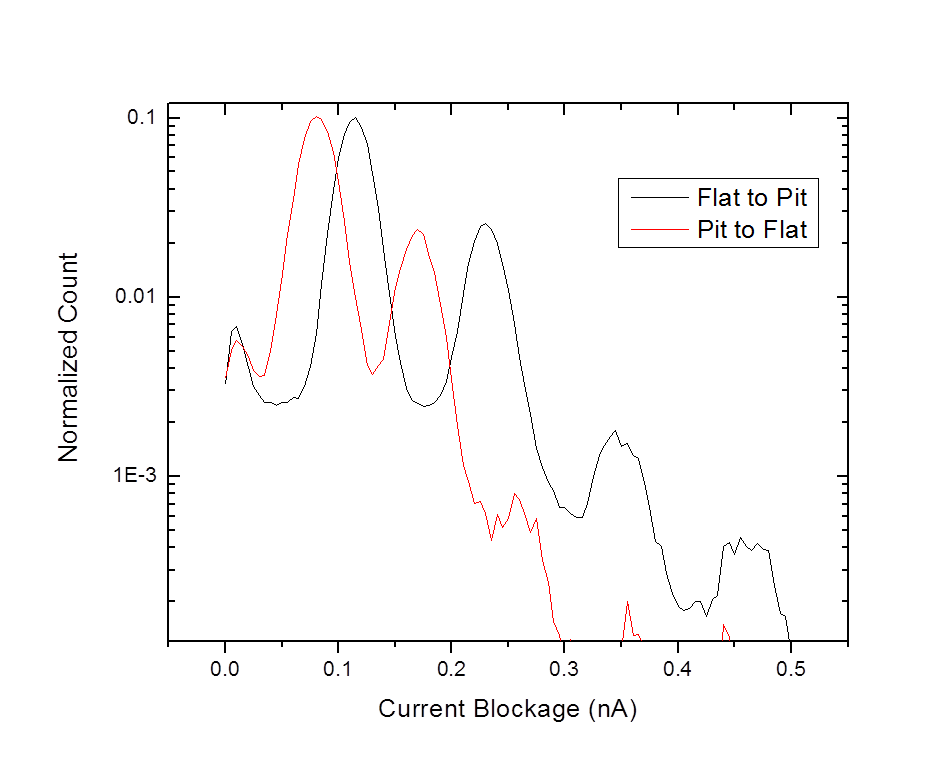
\includegraphics[width=.8\textwidth]{figures/blockage-histogram}
\caption{The histogram presented to the user to determine single-stranded current blockage.
The effect of the asymmetry of our structure is reflected in the differing current blockage values when translocations start from one side or the other.
The first two peaks are well-defined because many events have at least some portion where the molecule is folded once.
Higher numbers of folds are observed more rarely so the farther peaks are more poorly defined.}
\label{fig:blockage-histogram}
\end{figure}
We fit the histogram using a double-peaked Gaussian fit function and take the value of the first (and typically tallest) peak as the current blockage of a non-folded translocation.
We prompt the user to either agree that the peak value was properly fitted or to specify one.
We use that value to determine the other current blockage levels (which are linear with respect to number of folds) and run through all events as we ran through baseline, classifying them according to the pattern of levels.
The user then verifies that the given classification is correct, supplies one, or rejects the event.
The final step in event processing is calculating ECD, which is done by summing all data points in an event.
The rest of the pipeline takes analyzed data and creates graphs (making it useful but uninteresting technically).


\subsubsection{Ping-Pong Translocations}

The data analysis pipeline for ping-pong experiments proceeds largely as described above, but with more involved data sanitization and event detection.
\begin{figure}
\centering
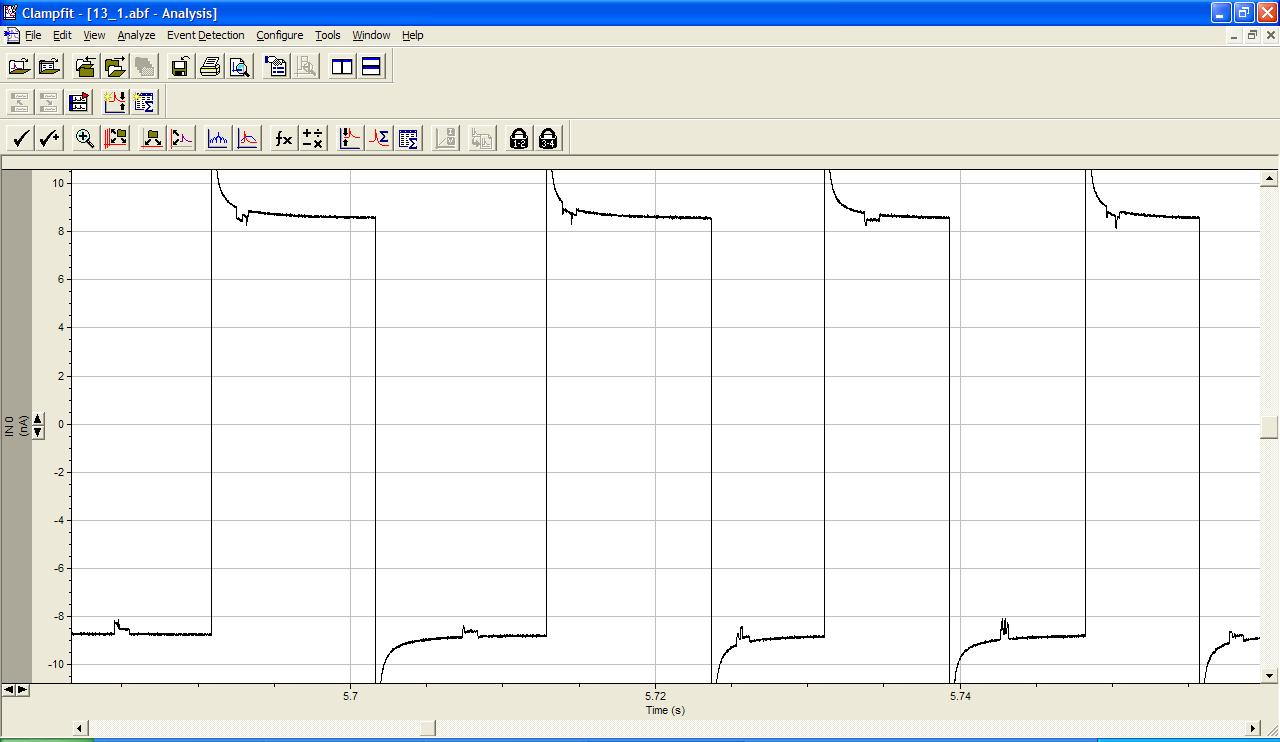
\includegraphics[width=1\textwidth]{figures/good-ping-pong}
\caption{A chunk of ping-pong data used to build our analysis algorithms.
Important features are the data's noisiness and translocations on moving baselines.}
\label{fig:good-ping-pong}
\end{figure}
The added complication is due to the nastiness of the data for which Fig.~\ref{fig:good-ping-pong} is a good representation.
Before we wrote code to detect and process events all analysis was hand-done, using voltage flips triggered by translocations to find events.
This analysis became increasingly arduous as noise increased, triggering false flips; flips were no longer a reliable indicator of a translocation and hours were wasted looking at empty baseline hunting for a single event.
Problematic features include, but are not limited to: increased noise in the data sets and translocations on moving baselines.

Moving baselines posed a huge problem because our only working automatic detection scheme relied upon a flat baseline and deviation from an average current value to detect an event.
This trigger was always firing because current was always moving, necessitating a brand new detection scheme.
Our first thought was to fit the exponential-seeming decay of the data and subtract it to allow us to use the same event detection method as for monodirectional translocations.
Fitting seemed ideal as it would best preserve ECD measurements, which was the end goal of that experiment: (to show that ECD is conserved, right?)
None of MatLab's fit functions worked when fed our data; either they over-fit and removed the event or they did not return a function at all.
We hypothesized that the sheer number of data points overwhelmed the fitting toolbox, so we tried sampling the data by averaging over various numbers of milliseconds.
Fitting still did not work.
Multiple problems arose while sampling, the greatest of which was that we would sample points within the event, pulling the fit function (if one was returned) into the event, destroying ECD measurements.
So we began fiddling with other possible heuristics for identifying events.

We eventually arrived at a robust heuristic to add to our detection arsenal by visual inspection of the data: use changes in the slope of the moving baseline.
Because the absolute value of slope is always decreasing on moving baselines, we used an increase in slope as our final test for event boundaries.
To find events, we first locate ``zaps'' in the data: places where the voltage flipped, causing a capacitive discharge that overloaded our recording equipment.
We run once through the data file, recording locations of all zaps.
We then search forward from the zap positions when searching for beginnings of events.
An event must pass a multi-step detection procedure to be classified as such.
First, we use our tried-and-true deviation from baseline current as a first flag.
However, we greatly reduce the number of data points used to define baseline current to 20 from 250 in the monodirectional case.
If lookahead current deviates far enough (defined on a per-dataset basis, typically around .15nA) from the baseline, we calculate a baseline slope value by finding the inter-data-point slopes (that is, the difference in current between adjacent data points) and averaging them.
We do the same for the lookahead data points.
If the lookahead average is greater than baseline average by .05nA/point (an arbitrary cutoff determined by lots of fiddling) we know we have found the beginning of an event.
Detection of event ends proceeds largely the same way except it looks backward from the next recorded zap. 

Noise was an issue because it would falsely trigger an event flag, causing junk to be processed, inducing human labor to manually clean data sets. 
[talk to mirna to fill in]

\section{Results and Discussion}

While I have no results in the classical experimental sense, my work at worst improved grad students' quality of life and at best will inform planning of future experiments.
Sarcasm aside, my major result is the method of automatic detection of translocations on a moving baseline.
[run through a minute of test data with script and by hand to see how many false positives there are]
The event pictured in Fig.~\ref{fig:tough-event} proved a particular problem for the script.
\begin{figure}
\centering
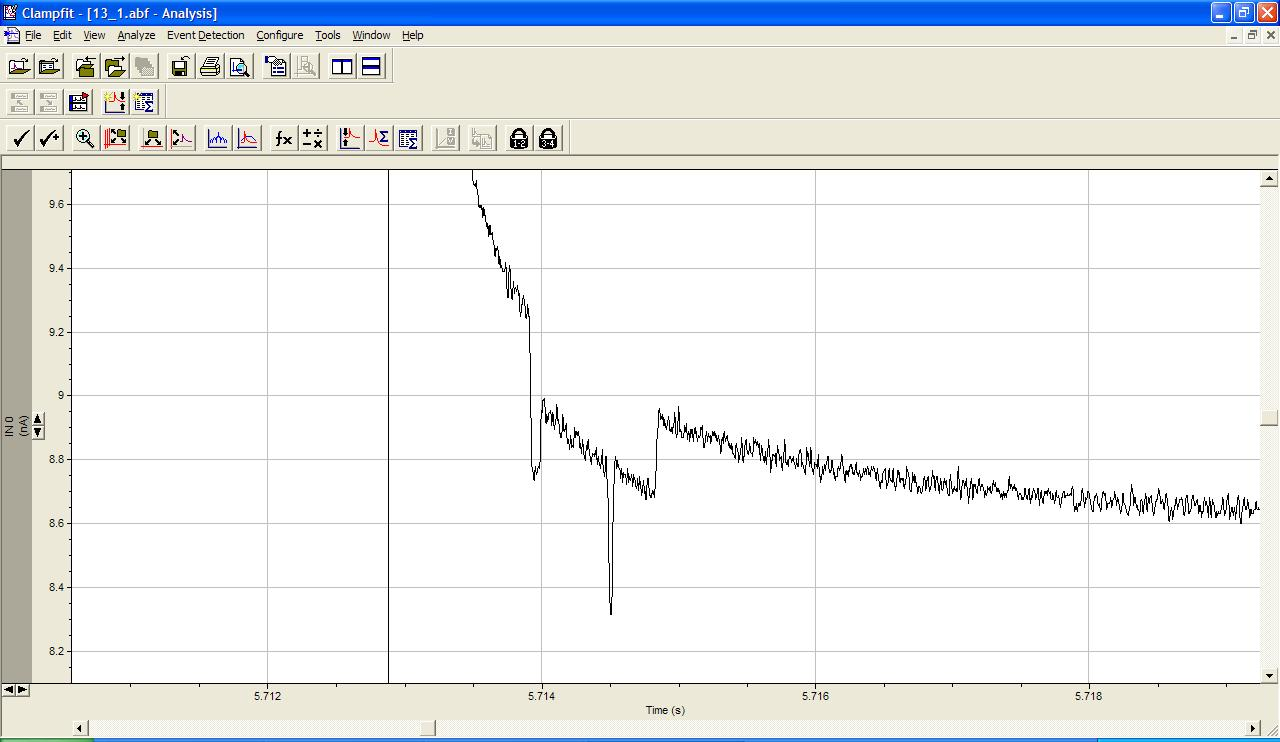
\includegraphics[width=1\textwidth]{figures/tough-event}
\caption{A particularly hard event to properly detect.
The folded-ness of translocation and location on decaying baseline proved particularly tough to interpret.}
\label{fig:tough-event}
\end{figure}
Most events are on less extreme slopes of baseline and do not have such unusual event structures.
Events like these forced me to reconsider my approach to event end detection multiple times
Adding that calculation to the FPGA's machine code will drastically reduce the number of voltage flips due to non-events.

One problem that still plagues monodirectional translocation analyses are ``spikes,'' small, unexplainable peaks that get flagged as events if the threshold is set low enough.
An example can be seen in \ref{fig:spike}.
Such false positives arise because the threshold for an event is set low enough that they get flagged.
Ultimately, the user decides this threshold and it is obvious that setting the threshold too low and getting false positives is better than setting it too high and missing events.
\begin{figure}
\centering
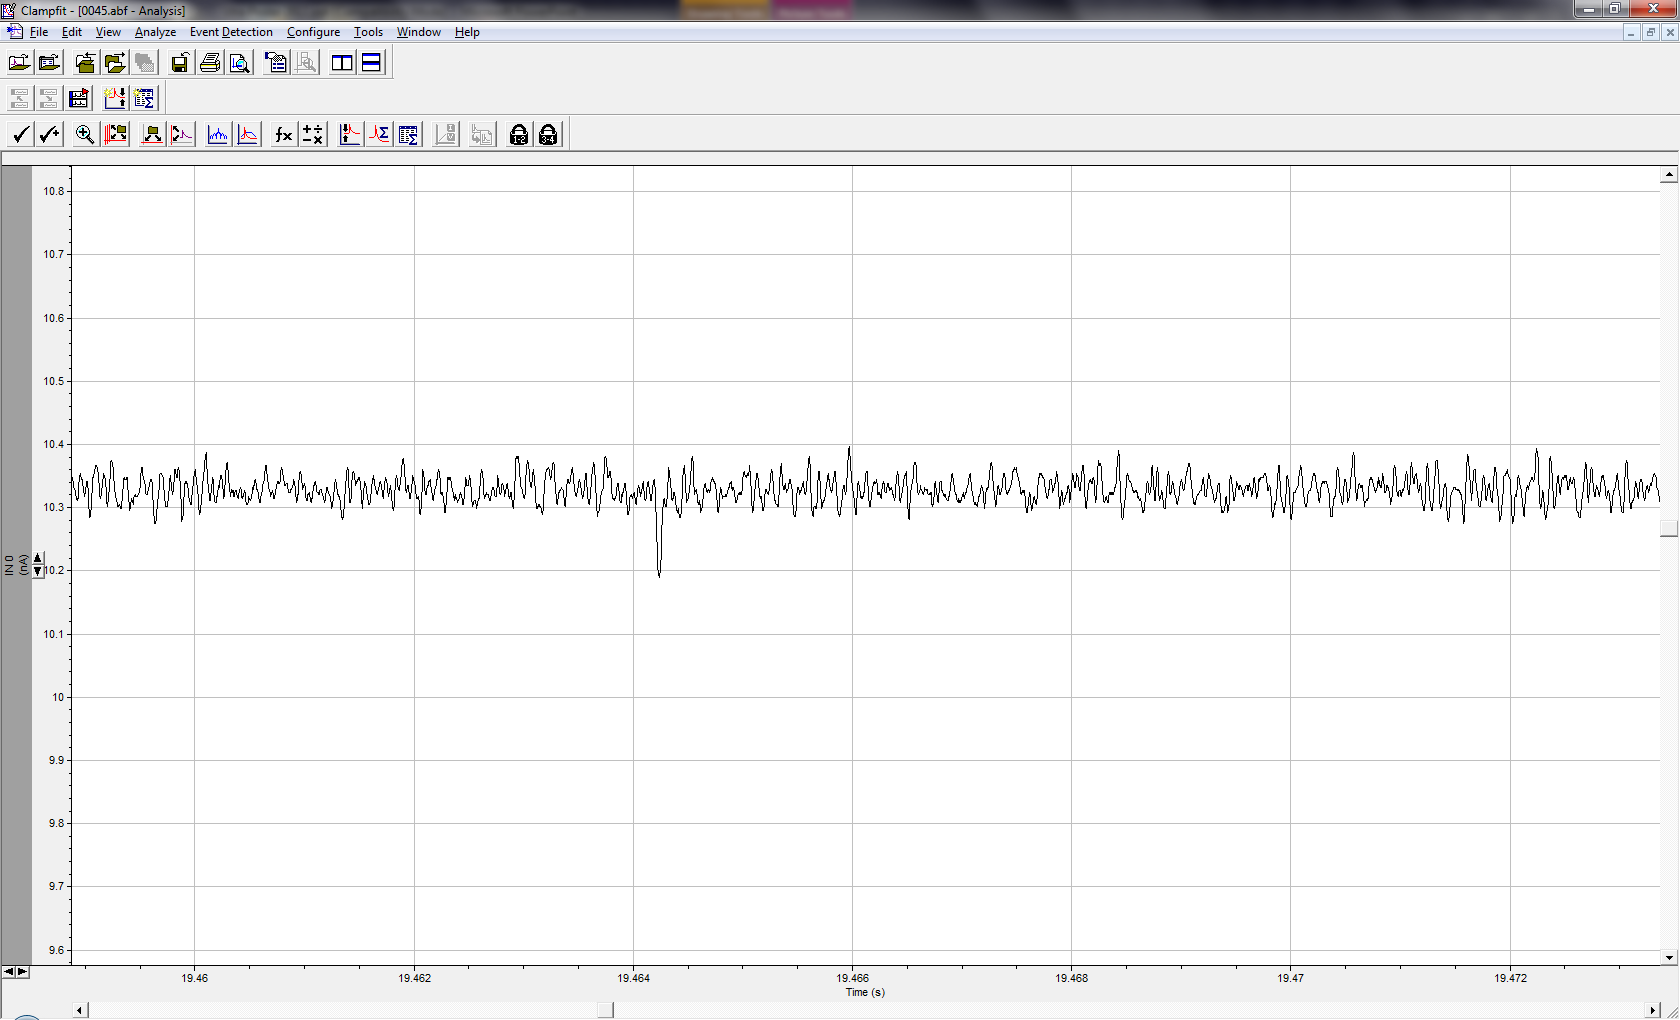
\includegraphics[width=1\textwidth]{figures/false-positive-example}
\caption{A small current spike that typically gets falsely flagged as an event.
The peak is approximately .11nA from the baseline, which is a reasonable cutoff for events.}
\label{fig:spike}
\end{figure}
The best and most straightforward way to avoid flagging spikes as events is to set a lower bound on event length.
We decided not to do so because that type of analysis treads dangerously close to falsely biasing our data.
Another method to combat such false positives is to offer some sort of suggested cutoff based on an analysis of the file.
The major problem with such an analysis is that very few things are constant over even a minute of data; the baseline can shift by a nanoamp or more, 


\section{Conclusion}

No longer will spurious translocations waste hours of labor

To improve upon the methods used in attempted trapping described above I offer two suggestions:
1) instead

% If in two-column mode, this environment will change to single-column
% format so that long equations can be displayed. Use
% sparingly.
%\begin{widetext}
% put long equation here
%\end{widetext}

% figures should be put into the text as floats.
% Use the graphics or graphicx packages (distributed with LaTeX2e)
% and the \includegraphics macro defined in those packages.
% See the LaTeX Graphics Companion by Michel Goosens, Sebastian Rahtz,
% and Frank Mittelbach for instance.
%
% Here is an example of the general form of a figure:
% Fill in the caption in the braces of the \caption{} command. Put the label
% that you will use with \ref{} command in the braces of the \label{} command.
% Use the figure* environment if the figure should span across the
% entire page. There is no need to do explicit centering.

% \begin{figure}
% \includegraphics{}%
% \caption{\label{}}
% \end{figure}

% Surround figure environment with turnpage environment for landscape
% figure
% \begin{turnpage}
% \begin{figure}
% \includegraphics{}%
% \caption{\label{}}
% \end{figure}
% \end{turnpage}

% tables should appear as floats within the text
%
% Here is an example of the general form of a table:
% Fill in the caption in the braces of the \caption{} command. Put the label
% that you will use with \ref{} command in the braces of the \label{} command.
% Insert the column specifiers (l, r, c, d, etc.) in the empty braces of the
% \begin{tabular}{} command.
% The ruledtabular enviroment adds doubled rules to table and sets a
% reasonable default table settings.
% Use the table* environment to get a full-width table in two-column
% Add \usepackage{longtable} and the longtable (or longtable*}
% environment for nicely formatted long tables. Or use the the [H]
% placement option to break a long table (with less control than 
% in longtable).
% \begin{table}%[H] add [H] placement to break table across pages
% \caption{\label{}}
% \begin{ruledtabular}
% \begin{tabular}{}
% Lines of table here ending with \\
% \end{tabular}
% \end{ruledtabular}
% \end{table}

% Surround table environment with turnpage environment for landscape
% table
% \begin{turnpage}
% \begin{table}
% \caption{\label{}}
% \begin{ruledtabular}
% \begin{tabular}{}
% \end{tabular}
% \end{ruledtabular}
% \end{table}
% \end{turnpage}

% Specify following sections are appendices. Use \appendix* if there
% only one appendix.
%\appendix
%\section{}

% If you have acknowledgments, this puts in the proper section head.
\begin{acknowledgments}
% put your acknowledgments here.
\end{acknowledgments}

% Create the reference section using BibTeX:
\bibliography{bibliogrpahy}

\end{document}
%
% ****** End of file template.aps ******
